% !TeX root = ../main.tex
\chapter{实验二:真实使用场景下的评测} %字符级别输入的部分
\label{cha:evaluation}
根据上一章的模拟结果,系统中集成了半键盘相对模型,作为单词级别输入的用户输入意图推理方法。此外,系统中还同时实现了字符级别输入。本章则主要介绍了整个系统的设计,并对单词级别输入、字符级别输入和混合模式输入三种使用场景做出用户评测以及相应的结果分析。

\section{平台设计}
% 平台图以及如何进行切换
\subsection{单词级别}
在单词级别的输入中,用户和实验一相同,将双手放置于手机前,在不显示键盘的情况下,按照自己的肌肉记忆在桌面上进行十指输入。

用户在进行输入时,平台的算法会根据用户点击的位置预测出用户可能的目标单词。屏幕上会显示出现概率最高的五个单词,用户可以使用右手右滑切换目标单词,和物理键盘相似,用户通过点击空格键选择当前光标的指向单词。如果用户认为自己输入出现错误,用户可以将左手左滑删除正在输入的部分或者删除上一个输入的单词。

\subsection{字符级别}
较为直观的输入字符的方式为显示完整键盘布局,用户移动到目标字符后进行选择。然而,由于手机的屏幕相对较小,且用户输入时眼部离手机有一定距离,因此若将所有字符完整显示在屏幕上不仅瞄准相对困难,且容易造成视觉疲劳。在单词级别输入时用户使用滑动的方式进行选择,因此字符级别的输入仍然采用类似的交互思路。

总体上系统使用二级菜单的设计,如图~\ref{fig:design}。其中第一级菜单为九宫格键盘,包括了26个英文字母和3个其他字符;当用户选择第一级菜单的某个方格之后,会出现二级菜单,二级菜单显示了对应方格的字符供用户进行选择。在一二级菜单中,用户均可以使用右手右滑向右移动光标,左手左滑向左移动光标以及任意手上滑 到达目标位置。仍然类似于单词输入,用户在一二级菜单进行选择时,可以使用右手任意手指进行点击。使用左手手指点击则对应退回的操作,如果当前在二级菜单则退回到一级菜单,如果在一级菜单则删除一个字符。

本系统还支持两种模式混合输入。用户通过点击离手机较远的位置(35cm之后)切换输入模式,实验一的数据表明,用户在正常输入时超过30cm的点击比例小于0.1\%,且最远为32cm。另外,用户能够很容易判断如何快速点击合适位置进行切换。

\begin{figure}[htbp] % use float package if you want it here
    \centering
    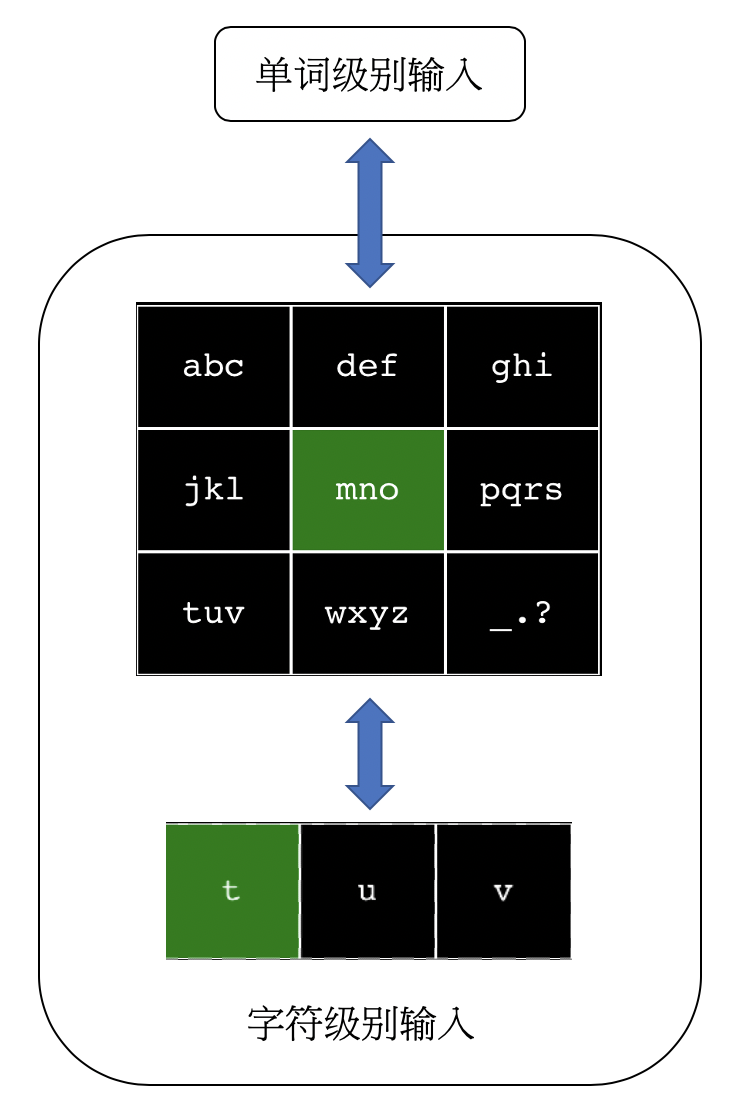
\includegraphics[height=11cm]{figures/design.png}
    \caption{平台设计结构图}
    \label{fig:design}
\end{figure}

\section{被试}
评测实验一共招募了3名被试。被试们平均年龄为21.67岁(标准差=0.58),且均熟练使用物理实体键盘。实验开始前,用户仍然先使用了TextTest\cite{texttest}\cite{wobbrock2006analyzing}测试在物理键盘的输入速度。他们平均速度达到了59.3单词每分钟(标准差=8.86),无纠正错误率为0.06\%(标准差=0.04\%)。

\section{实验装置和实验平台}
本次实验的装置和实验一相同。实验平台同样类似,但是显示了当前的输入模式,在单词输入模式下多了一行单词供用户进行选择,在字符输入模式下显示一级或者二级菜单,见图~\ref{fig:platform1}。

\begin{figure}[h]
  \centering%
  \subcaptionbox{单词模式输入\label{fig:platform11}} %标题的长度,超过则会换行,如下一个小图。
    {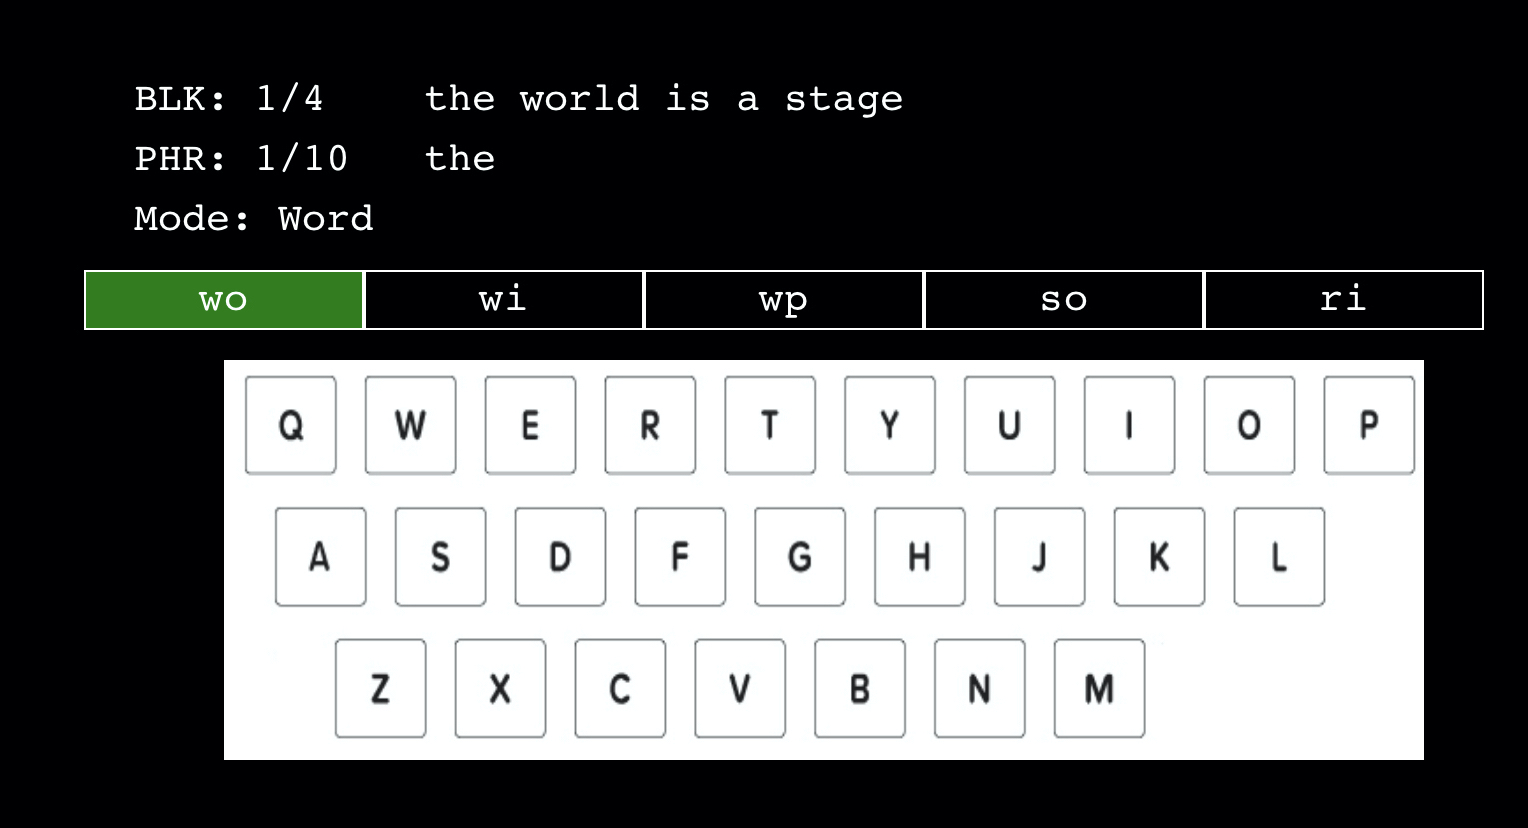
\includegraphics[height=5cm]{figures/platform11.jpg}}%
  \hspace{4em}%
  \subcaptionbox{字符模式输入\label{fig:platform12}}
      {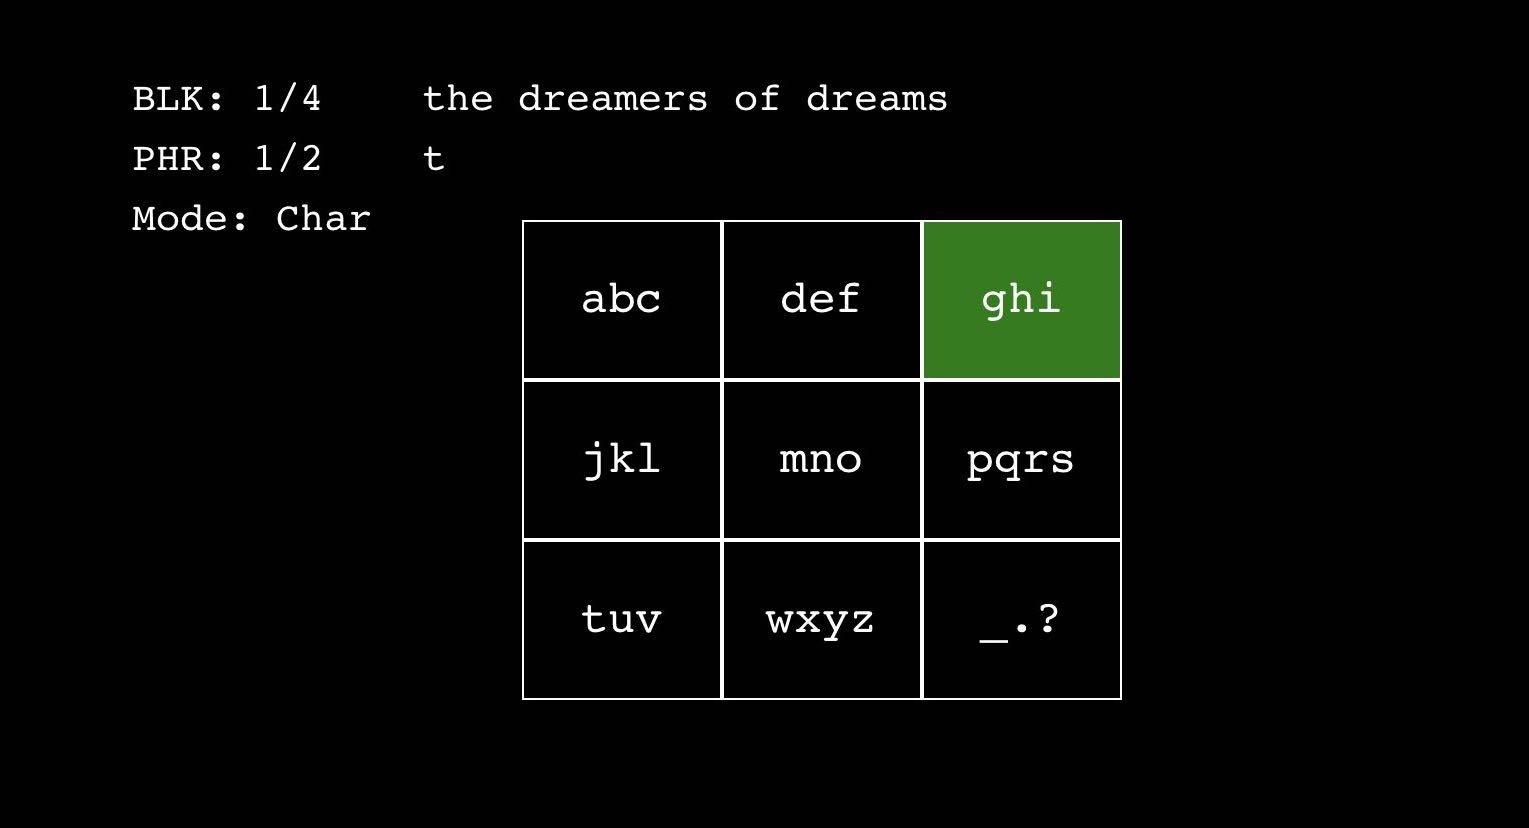
\includegraphics[height=5cm]{figures/platform12.jpg}}
  \hspace{4em}%
  \subcaptionbox{混合模式输入\label{fig:platform13}}
      {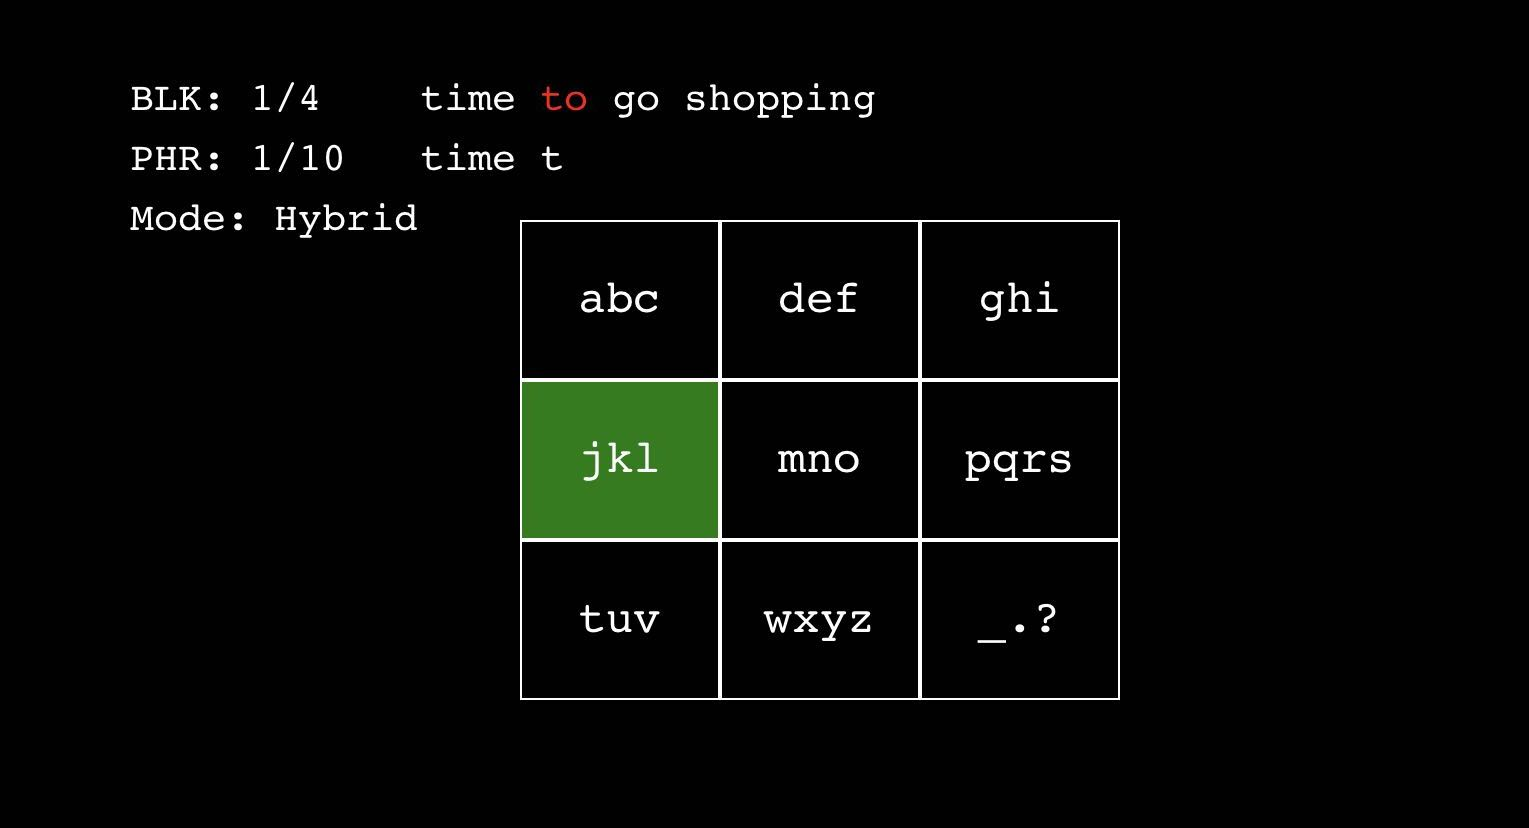
\includegraphics[height=5cm]{figures/platform13.jpg}}
  \caption{实验二平台截图}
  \label{fig:platform1}
\end{figure}


% \begin{figure}[h] % use float package if you want it here
%     \centering
%     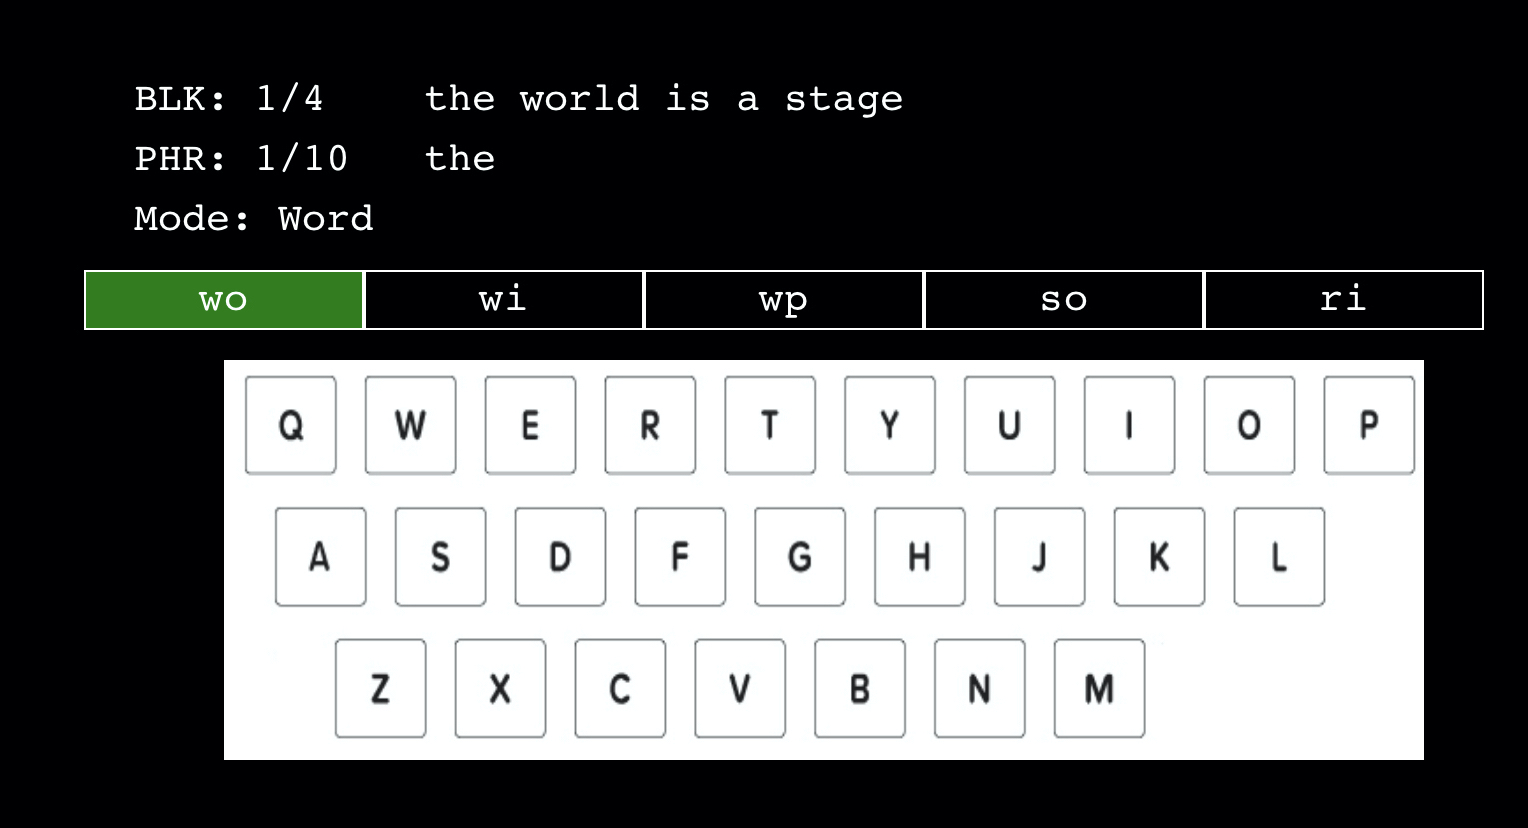
\includegraphics[height=5cm]{figures/platform11.jpg}
%     \caption{实验二平台截图}
%     \label{fig:platform1}
% \end{figure}

\section{实验设计和流程}
为了研究平台在不同情况下的输入效率,评测实验分为三个模式,分别是单词模式、字符模式和单词字符混合模式。具体操作方式见本章平台设计部分。为了避免不同模式顺序对结果的影响,每位用户实验时先进行单词模式和字符模式输入,两者顺序随机,最后进行混合模式输入。屏幕上会标明当前的输入模式。在用户输入单词时,词库大小为10,000个单词,和第~\ref{cha:sensing}~章相同。

在单词模式和混合模式的输入中,用户需要完成4个输入块,每个输入块10句话,为Mackenzie句库随机选择而成\cite{mackenzie2003phrase}。其中混合模式下,每个句子中随机选择一个单词标红,用户必须通过逐个输入字符的方式拼出该单词,其余的部分则仍然输入整个单词。在字符模式下,用户同样完成4个输入块,每个输入块2句话,也为Mackenzie句库\cite{mackenzie2003phrase}打乱并挑选构成。为了使用户使用时更清晰方便,输入字符时使用'\_'表示空格。

在正式实验开始前,每位用户有10分钟的时间熟悉实验平台。用户需要尽可能速度快且准确地输入每一句话。每当用户输入完一个句子后,他们可以点击任意按键跳到下一句。在输入块之间,用户需要强制休息2分钟。在完成一句后,用户也可以根据个人需求将手放在桌面上休息。实验结束后,用户需要填写一个问卷用于收集相关信息。

在评测中,输入速度的计算仍然使用公式~(\ref{equ:calcspeed})。而CER\cite{cer},即字符级别准确率被用来衡量用户输入的准确性。CER表示将用户输入的字符串改成目标句子需要的最少的删除、增加、替换操作总次数除以目标句子长度。当CER越接近1时,则输入准确性越高。对于每个句子,文章分别计算CER,最后取平均值。另外,本文使用RM-ANOVA进行相关的数据分析,将$p<.05$的结果视为显著。

\section{字符模式输入}
% 在字符模式的输入中,用户同样完成4个输入块,每个输入块2句话\cite{mackenzie2003phrase},为Mackenzie句库随机挑选构成。

\begin{figure}[h]
  \centering%
  \subcaptionbox{字符模式输入速度\label{fig:charspeed}} %标题的长度,超过则会换行,如下一个小图。
    {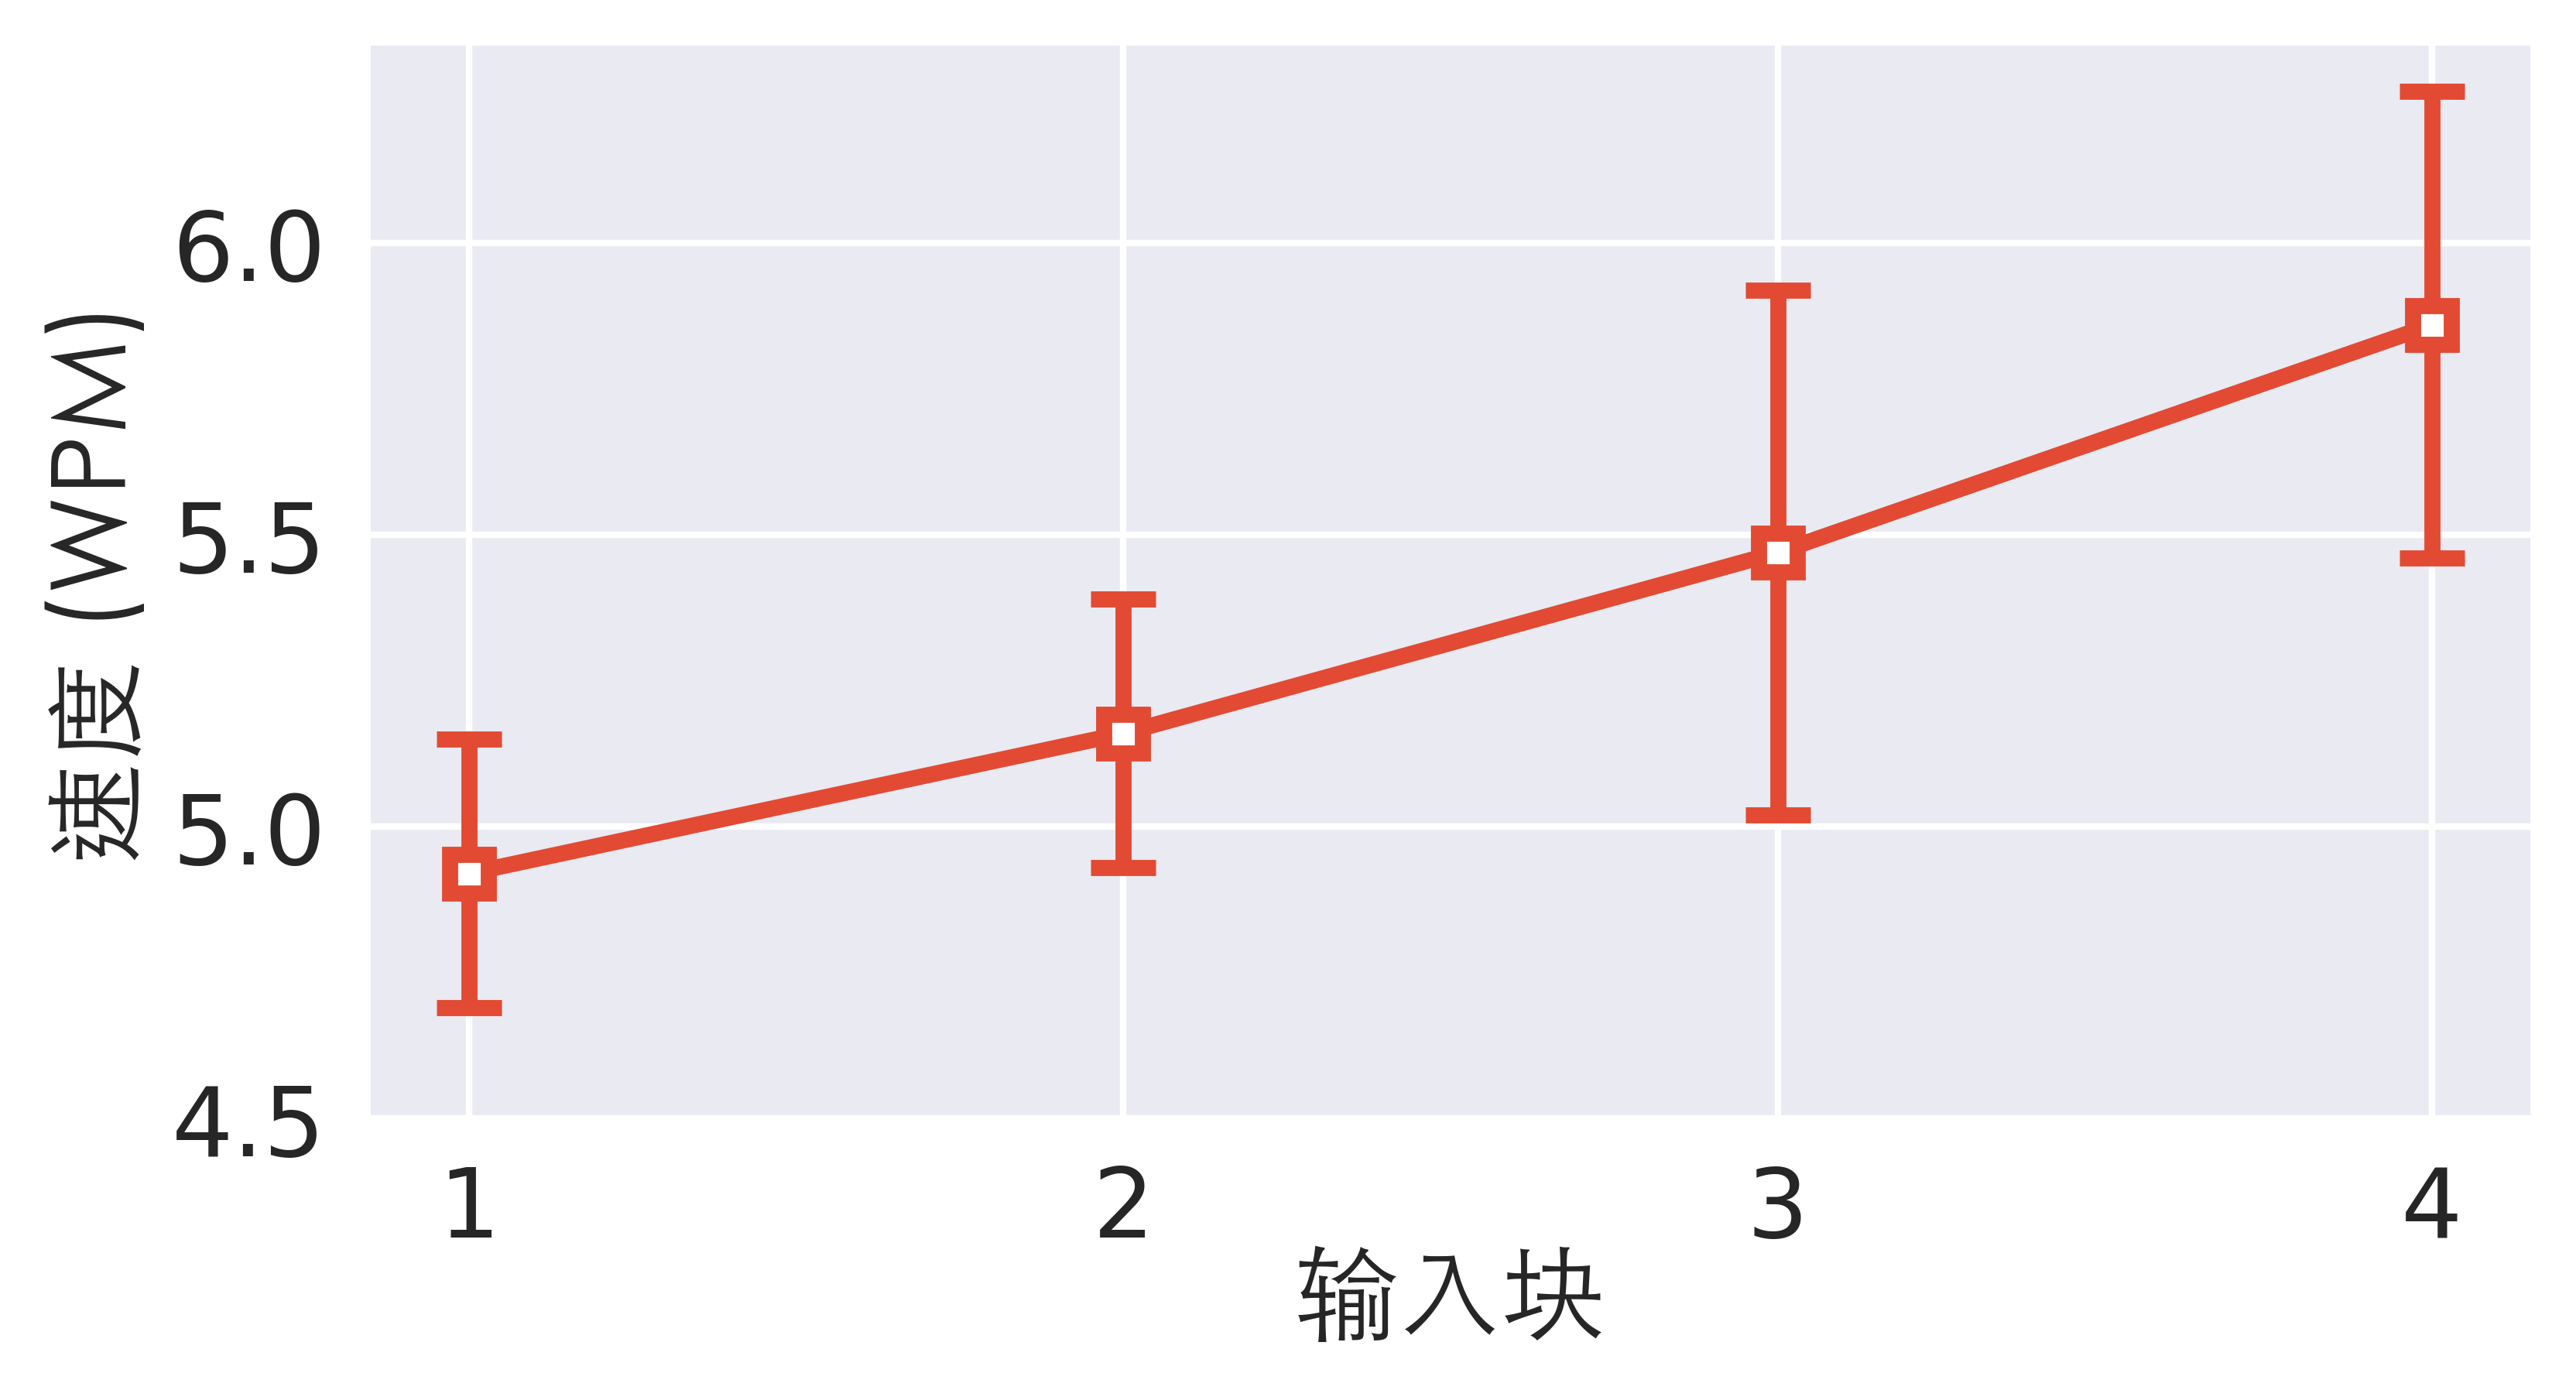
\includegraphics[height=3.5cm]{figures/charspeed.png}}%
  \hspace{4em}%
  \subcaptionbox{字符模式操作次数\label{fig:charops}}
      {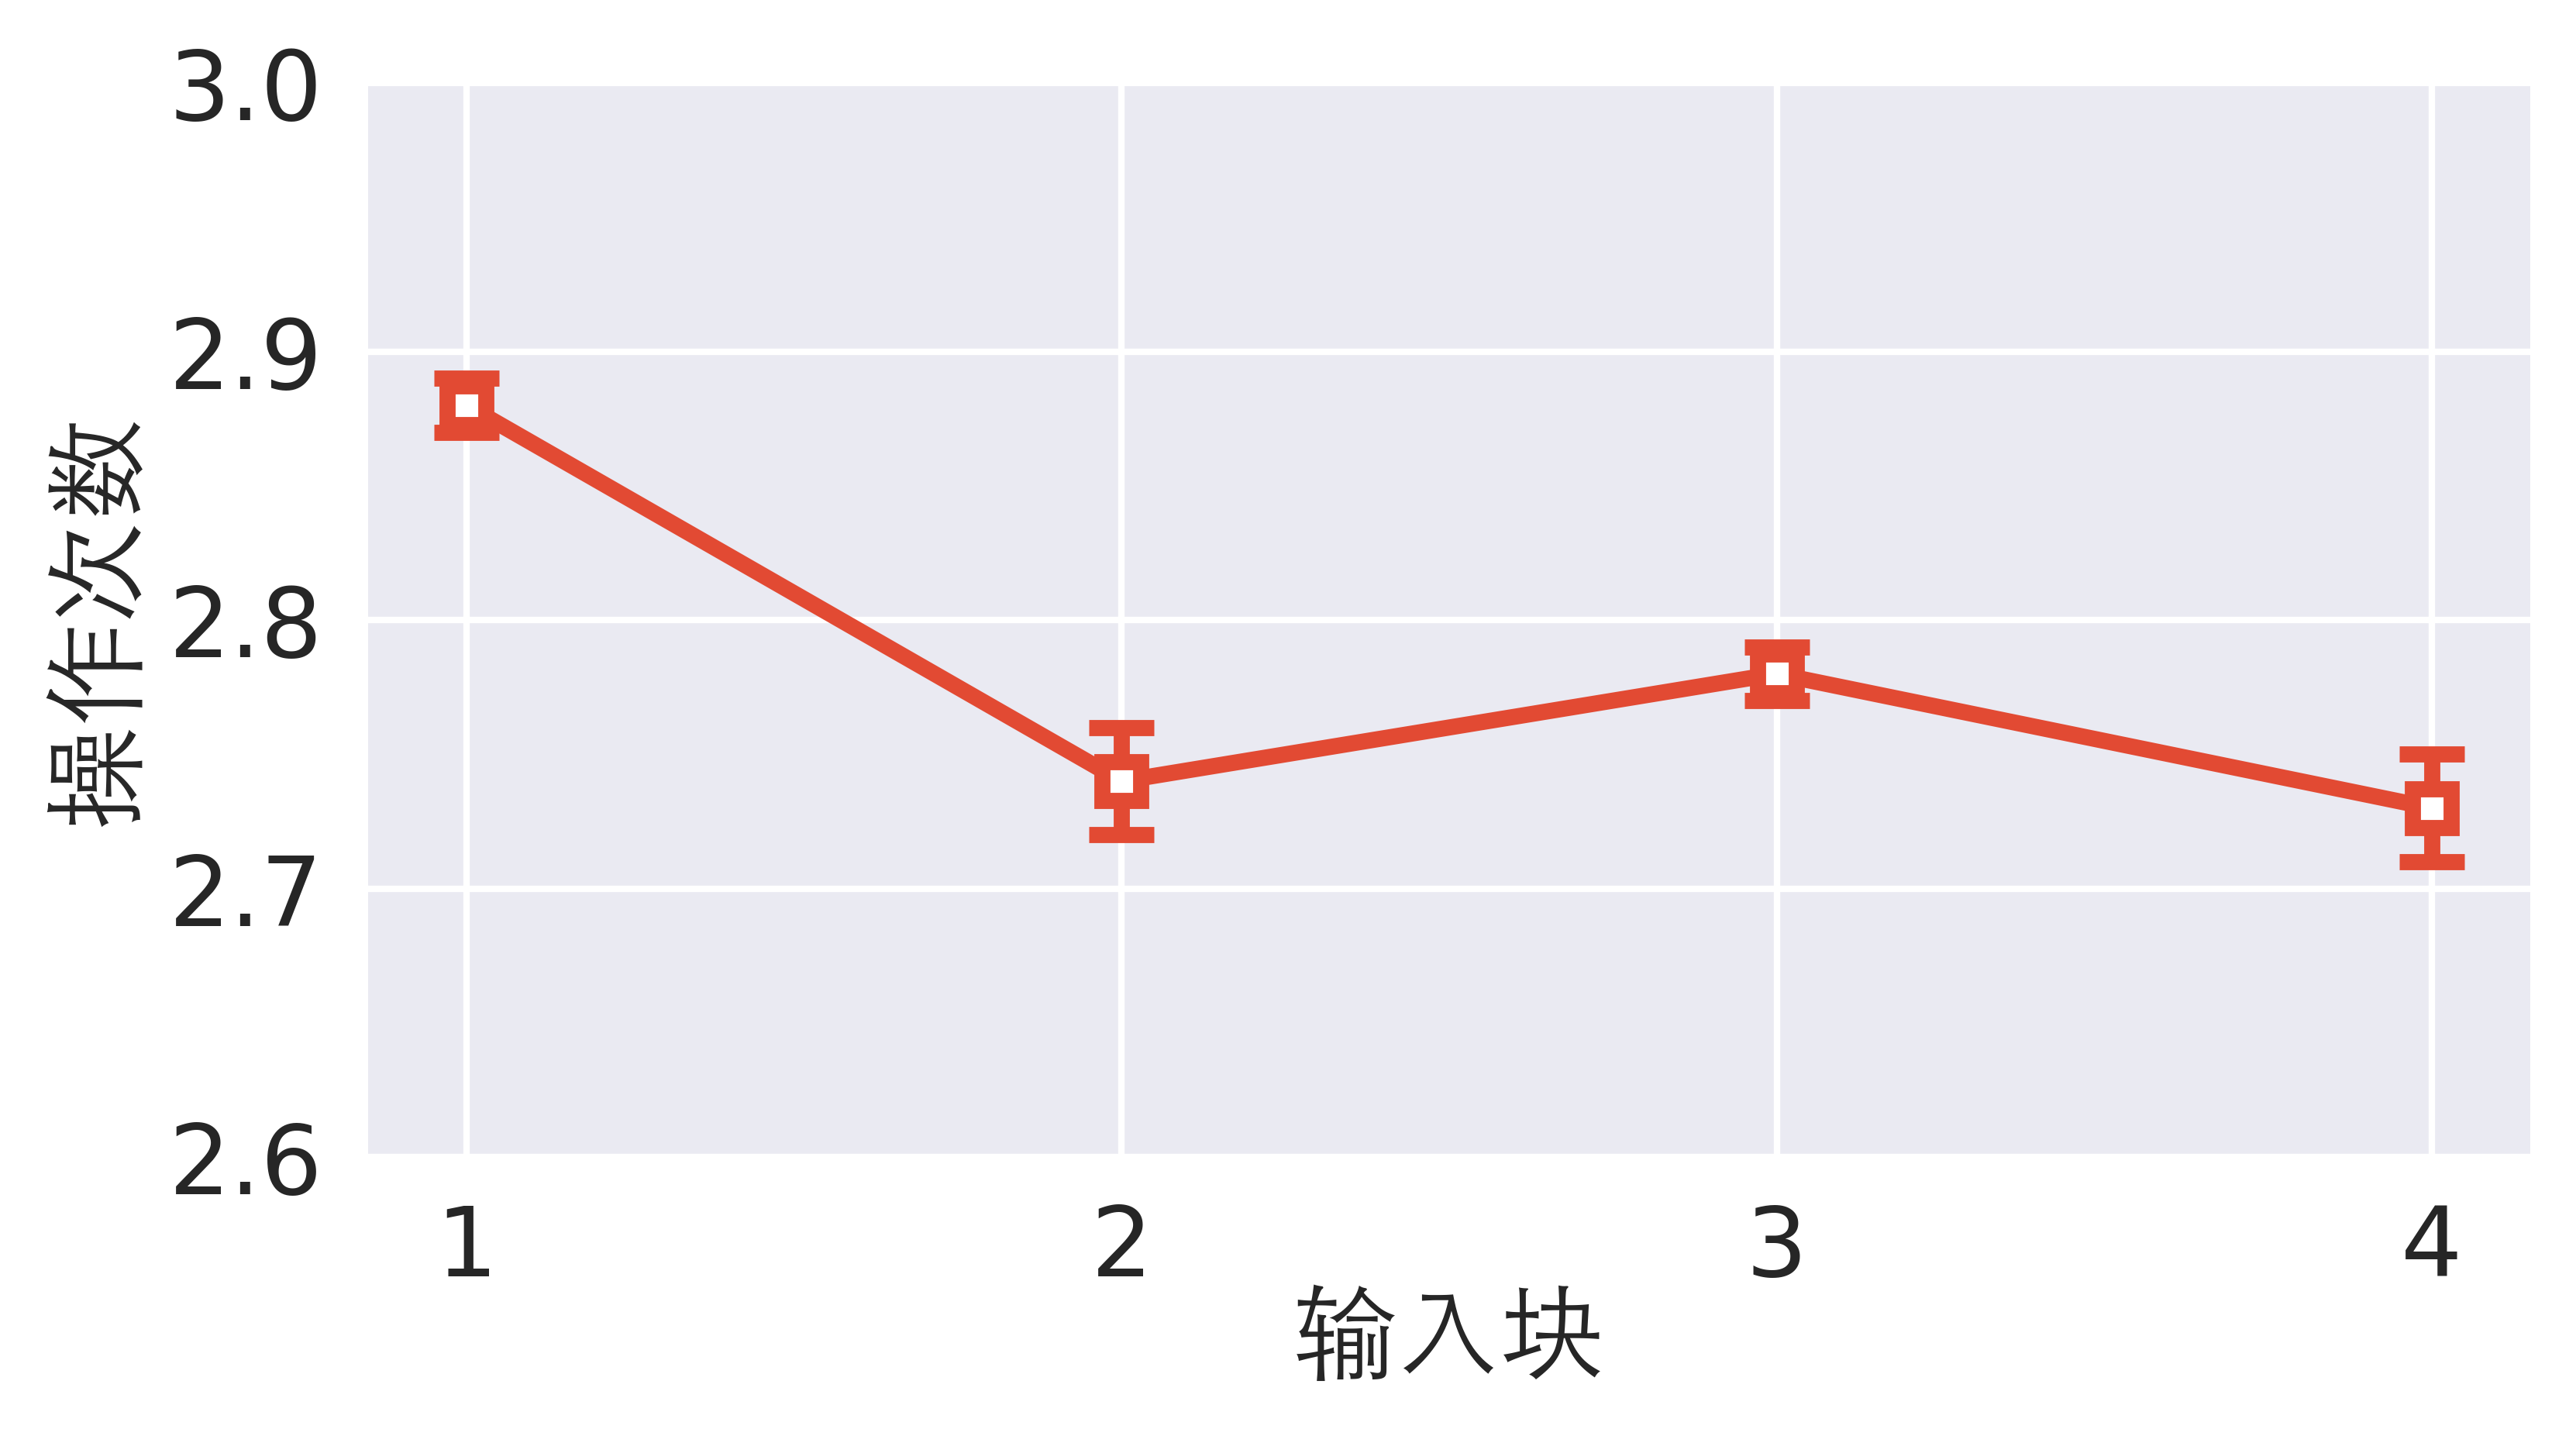
\includegraphics[height=3.5cm]{figures/ops.png}}
  \caption{字符模式速度和操作次数,误差棒为一标准差}
  \label{fig:charres}
\end{figure}

字符模式下,平均输入速度为5.36WPM(标准差=0.47),快于手机上控制一维光标或者二维触摸屏划分区域进行输入字符的速度\cite{2018forceboard}\cite{1dhandwriting}。本文还计算了用户每个输入块的平均操作次数,即上滑、左滑右滑次数。操作次数平均为2.68(标准差=0.18)。输入速度和($F_{4,8}=5.06, p < .05$)操作次数($F_{4,8}=36.62, p < .001$)和输入块显著相关,说明用户能够逐渐熟练掌握二级菜单输入字符的方法,这一点从从图~\ref{fig:charres}也可以看出。

字符模式输入下,输入块和CER关系不显著($F_{4,8}=0.38, p =0.77$),并且CER维持在较低的水平,平均为1.4\%(标准差=1.1\%)。原因在于用户逐个输入字符出错概率较低,即使出错也会重新输入。

\section{单词模式输入}

\subsection{输入速度}
用户在输入单词时的平均速度为40.32WPM(标准差=3.40),输入速度随着输入块增加,在最后一个输入块的平均速度为44.19WPM,该速度与触摸屏上十指盲打基本一致\cite{2018shitoast},慢于在物理键盘上的速度。输入速度和输入块显著相关($F_{4,8}=59.78, p < .001$)。

\subsection{输入准确性}

在单词输入模式中,CER整体平均值为0.37\%(标准差=0.42\%),与输入块的关系不显著($F_{4,8}=2.70, p =0.14$)。总体来看,CER仍然处于较低的水平,原因有两点,一是输入推理算法准确性较高,能够预测用户的目标单词;二是即使用户点错位置或者选择了错误的单词,通常会选择重新进行输入。

\subsection{用户行为数据}
本文对于用户在单词级别输入时的交互数据也作出了统计,其中“单词一匹配”表示用户选择了出现的第一个单词,且该单词与目标句子对应单词相同,“单词一不匹配”则表示选择单词一但是该单词错误;以此类推,“非单词一匹配”和“非单词一不匹配”分别表示用户选择的单词不是第一个时,该单词正确与否的情况。“撤销”操作表示用户未输入完一个单词时清空当前的输入内容;“删除”则表示用户删除输入框中一个单词,一般为选择了错误的单词后删除重新输入。

\begin{table}[h]
  \centering
  \begin{minipage}[t]{0.9\linewidth} % 如果想在表格中使用脚注,minipage是个不错的办法
  \caption[单词模式下用户各行为百分比]{单词模式下用户各行为百分比}
  \label{tab:word-stat}
    \centering
    \begin{tabularx}{\linewidth}{cccccc}
      \toprule[1.5pt]
      %  & \multicolumn{2}{c}{总体}&\multicolumn{2}{c}{左手} &  \multicolumn{2}{c}{右手} \\\midrule[1pt]
      单词一匹配 & 单词一不匹配 & 非单词一匹配 & 非单词一不匹配 & 删除 & 撤销\\\midrule[1pt]
      72.10 & 2.74 & 20.81 & 0.65 & 2.10 & 1.61\\
      \bottomrule[1.5pt]
    \end{tabularx}
  \end{minipage}
\end{table}

从表格~(\ref{tab:word-stat})可以看出,用户的绝大部分操作为“单词一匹配”(72.10\%),说明算法能够很好预测用户的目标单词。不匹配的情况大部分出现在选择单词一时,表示用户输入完成一个单词直接点击确定,造成输入错误,然后用户会将该单词删除重新输入,类似在物理键盘上的行为。该行为从侧面反应用户较为熟练且信任本技术的使用方法。


\section{混合模式输入} 

\subsection{输入速度}
用户在混合模式下,整体的输入速度为17.63WPM(标准差=1.93),该速度快于智能手表的输入技术\cite{compass},稍慢于手机单手输入\cite{2017blindtype}。然而,这里提到的这两种输入方式都仅为单词输入,而本文在混合模式下输入即能达到该速度,证明了技术的实用性。另外,输入单词的平均速度为40.25WPM(标准差=2.80),输入字符的平均速度为5.10WPM(标准差=0.39)。不同输入块差距不明显(输入单词时$F_{4,8}=1.49, p =0.30$,输入字符时$F_{4,8}=0.82, p =0.52$),表明在经过前面两个模式的实验之后,用户以及较为熟悉了对应的输入方法。在混合模式下,输入单词和字符的速度较单独输入有所下降,说明用户在切换模式时需要一定时间进行调整。

\begin{figure}[h] % use float package if you want it here
    \centering
    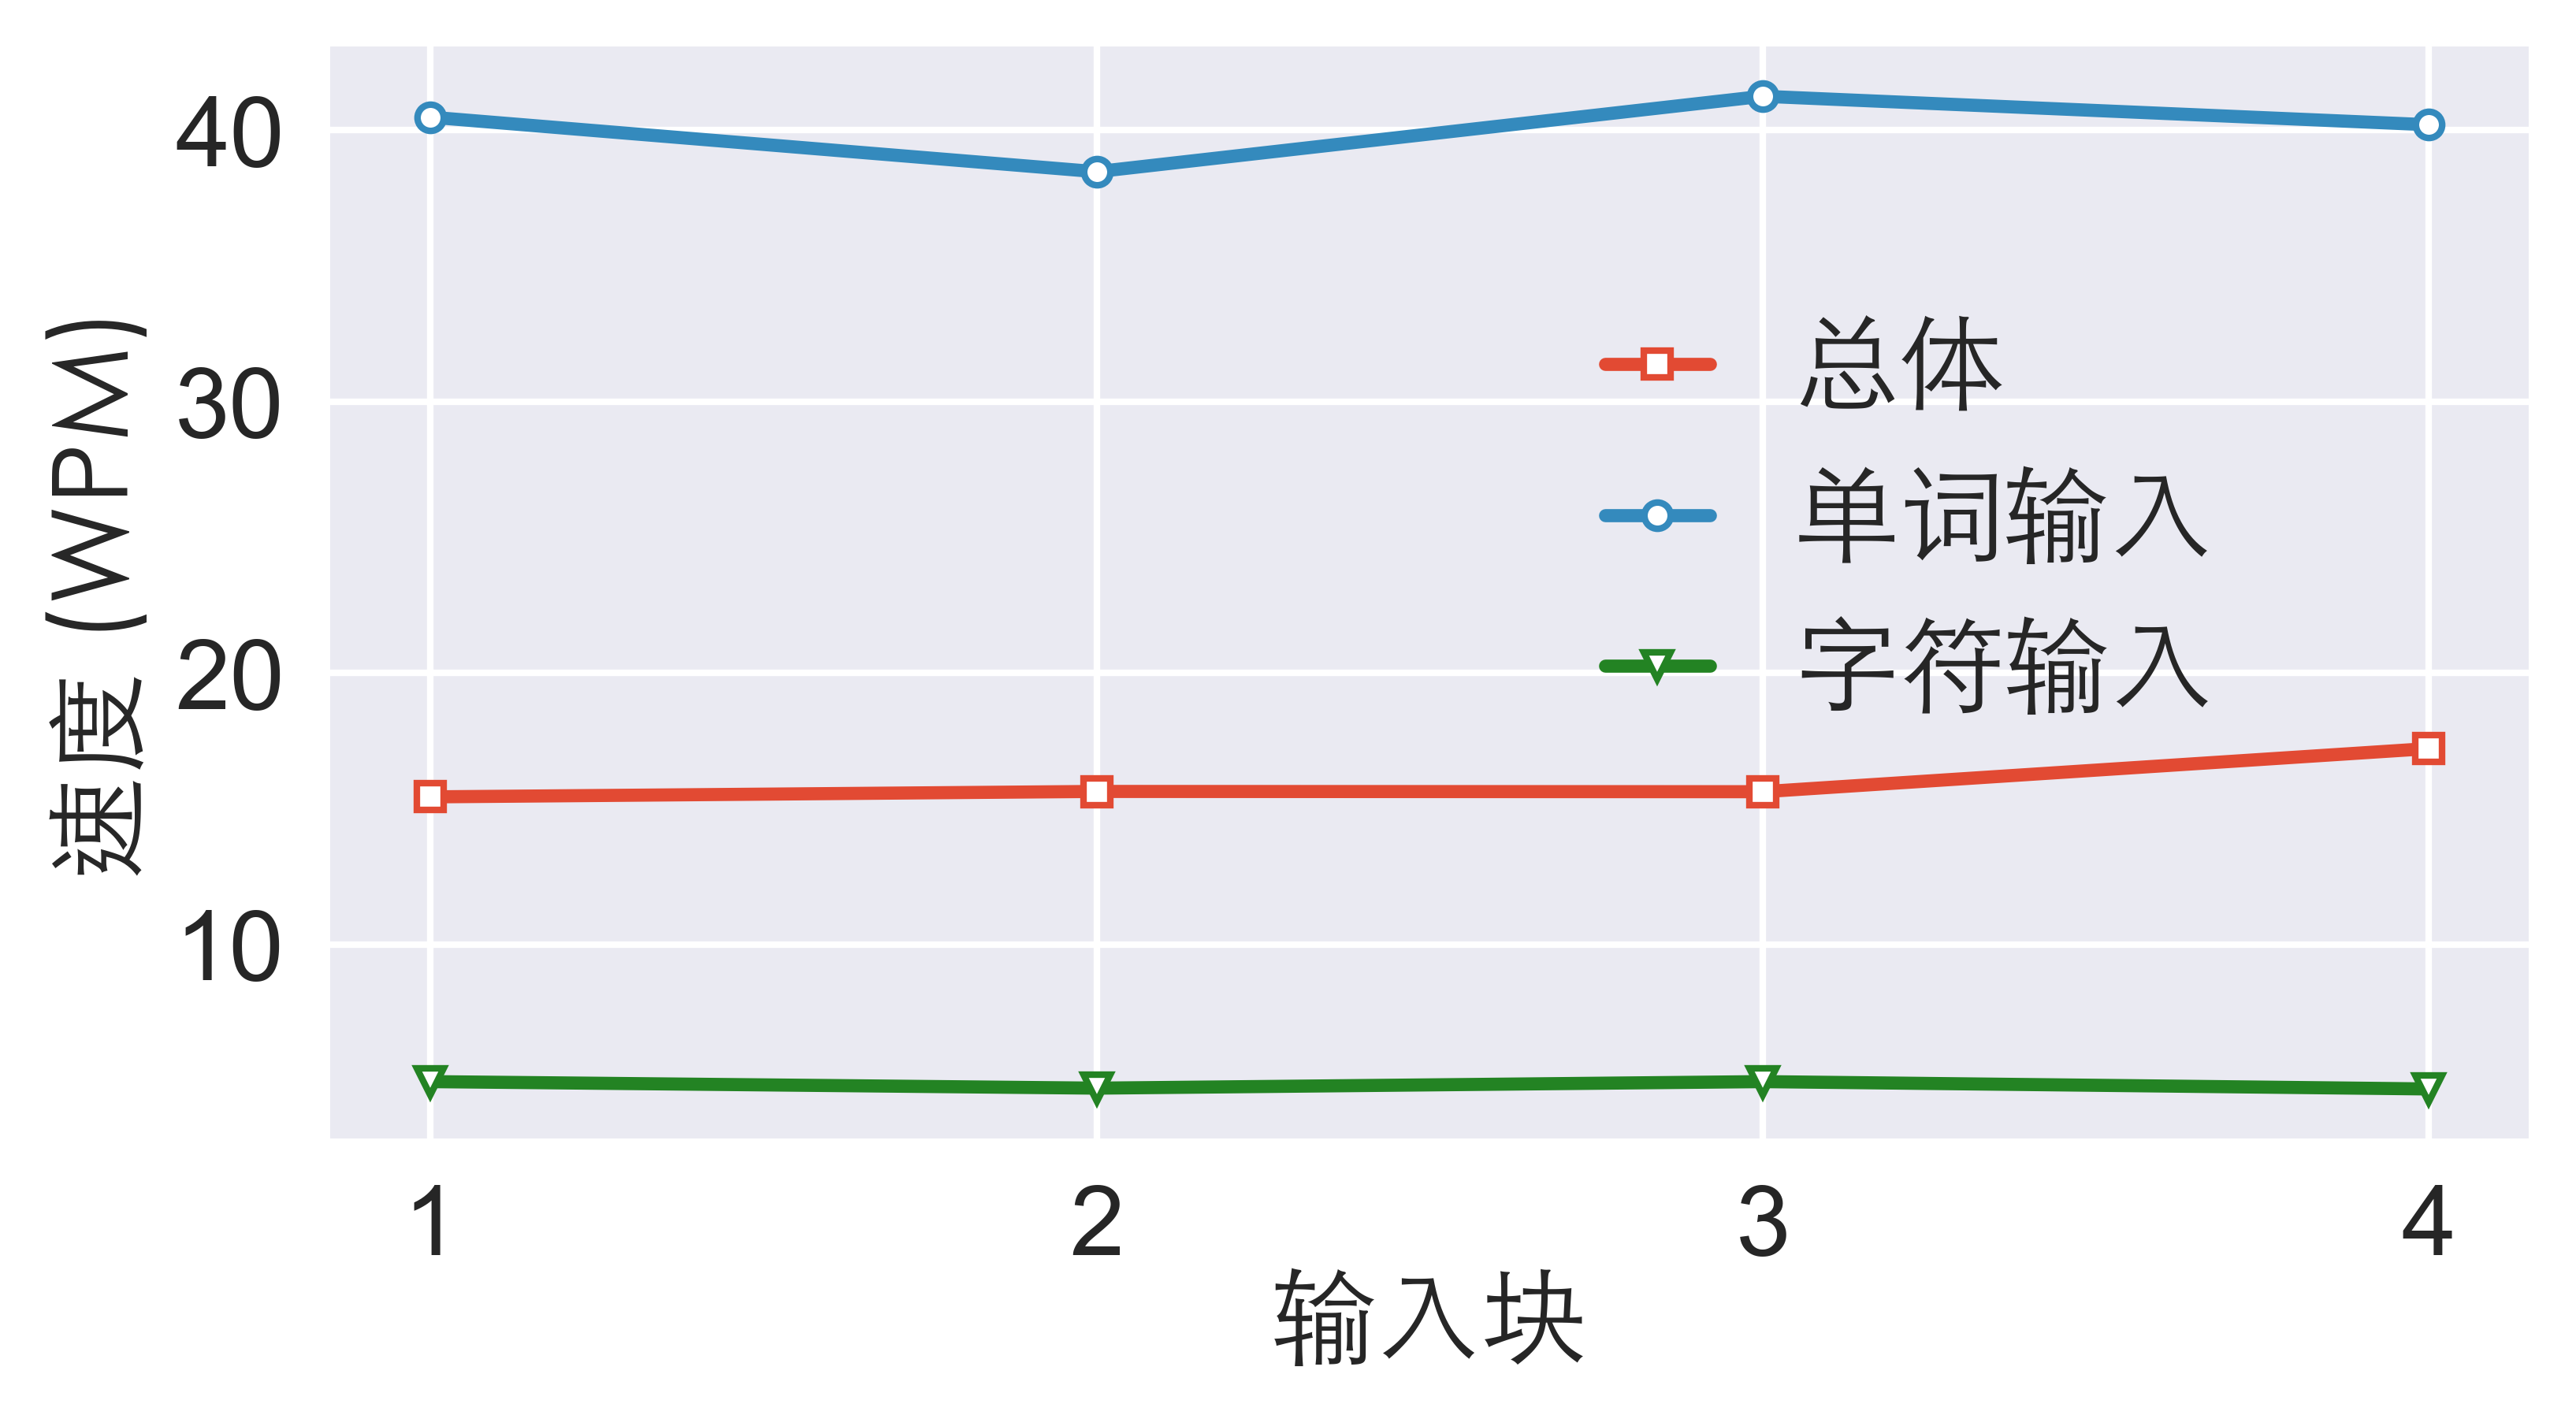
\includegraphics[height=5cm]{figures/wholespeed.png}
    \caption{混合模式输入速度,误差棒为一标准差}
    \label{fig:wholespeed}
\end{figure}


\subsection{输入准确性}
用户的输入准确性较高,总体、输入单词、输入字符的CER分别为0.6\%(标准差=0.3\%),0.7\%(标准差=0.6\%),0.9\%(标准差=1.1\%),均与输入块无明显相关性。

\subsection{用户行为数据}
用户在输入字符时的平均操作次数为2.72(标准差=0.21),和单独输入字符时基本一致,说明混合输入对用户输入字符的行为影响不大。操作次数和输入块无明显关联($F_{4,8}=0.91, p =0.48$)。

和单词模式输入相同,文章同样统计了用户在输入单词时的交互行为数据,如表~\ref{tab:hybrid-stat}。“单词一匹配”的百分比有所下降,对应的“非单词一匹配”的百分比上升,说明用户在混合模式下输入准确性有所下降,可能为输入字符前后手的位置有所变化造成了点击准确度降低。

\begin{table}[h]
  \centering
  \begin{minipage}[t]{0.9\linewidth} % 如果想在表格中使用脚注,minipage是个不错的办法
  \caption[混合模式下用户输入单词各行为百分比]{混合模式下用户输入单词各行为百分比}
  \label{tab:hybrid-stat}
    \centering
    \begin{tabularx}{\linewidth}{cccccc}
      \toprule[1.5pt]
      %  & \multicolumn{2}{c}{总体}&\multicolumn{2}{c}{左手} &  \multicolumn{2}{c}{右手} \\\midrule[1pt]
      单词一匹配 & 单词一不匹配 & 非单词一匹配 & 非单词一不匹配 & 删除 & 撤销\\\midrule[1pt]
      69.97 & 3.86 & 24.52 & 0.00 & 1.1 & 0.51\\
      \bottomrule[1.5pt]
    \end{tabularx}
  \end{minipage}
\end{table}

\section{本章总结}
本章详细介绍了输入系统的具体实现,并且对提到的三种输入模式分别进行了用户评测。结果表明,用户使用本系统输入单词的速度能够超过40WPM,输入字符的速度超过5WPM,并且在混合输入时速度接近18WPM。在保证速度的同时用户们也能够维持较高的输入准确性。实际使用场景下的用户实验证明了本输入技术的高效性和实用性。
